\documentclass[a4j,12pt,landscape]{jarticle}
\topmargin=3mm \headheight=0mm \headsep=0mm
\textheight=170mm 
\textwidth=220mm
\evensidemargin=0mm \oddsidemargin=0mm
\footskip=0mm
\parindent=0cm

%\usepackage[all]{xy}
\usepackage{amssymb}
\usepackage{amscd}
\usepackage{amsmath}
\usepackage{graphics}
\usepackage{graphicx}
\usepackage{amsthm}

\pagestyle{empty}

\def\modulo{{\rm mod}}
\def\F2{{\mathbb F}_2}
\def\wt{{\rm wt}}
\def\wo{{\rm wt}_o}
\def\wf{{\rm wt}_f}
\def\UL{{\rm ul}}
\def\bx{{{\mathbf x}}}
\def\by{{{\mathbf y}}}
\def\bw{{{\mathbf w}}}
\def\bu{{{\mathbf u}}}
\newcommand{\lshift}[1]{{\large $\mbox{#1}\atop<<$}}
\newcommand{\rshift}[1]{{\large $\mbox{#1}\atop >>$}}

\title{}
\author{}
\date{\today}

\begin{document}
\Huge

\vspace*{2cm}
\begin{center}
{\bf Simple and Fast MT:\\
  A Two times faster new variant of Mersenne Twister}
\vspace{1cm}

Mutsuo Saito (Hiroshima Univ.) \\
and \\
Makoto Matsumoto (Hiroshima Univ.).
\end{center}
\vspace{\fill}
This research is granted by 
\newpage

\newpage
\noindent
{\bf 1. Pseudo Random Number Genarator}\\

In this talk, PRNG is a (finite state) automaton consisting of:
\begin{itemize}
\item State set $S$. 
\item Transition function $f:S \to S$.
\item Initial state $s_0 \in S$.
\item (No imput considered.)
\end{itemize}
Change the state as follows:
$$
s_0 \mapsto s_1:= f(s_0) \mapsto s_2:=f(s_1) \mapsto \cdots.
$$

\newpage
Let $O$ be the set of output symbols.

(In this talk, we assume $O$=32-bit integers.)

\vskip 1cm
At each state $s$, 
the output is determined by 
\begin{itemize}
\item an output function $o:S \to O$.
\end{itemize}
The output sequence becomes
$$
o(s_0),o(s_1),o(s_2),\ldots.
$$
We use this as a pseudo-random sequence.
\newpage
\begin{center}
\includegraphics[width=0.7\linewidth]{figure01.eps}
\\
Figure 1: Automaton.
\end{center}

 
\newpage
\noindent
{\bf 2. Feedbacked Shift Regiter}\\
In the above automaton, 
its period is bounded  \\
by the number of the states $\#(S)$.

\vskip 5mm
We want large $S$ (like 20000 bits), \\
which admits fast computation of $f$ \\
in a software implementation.

\vskip 5mm
Feedbacked Shift Register (FSR) permits $f$ \\
with $O(1)$-time complexity.

\newpage
Feedbacked Shift Register.
\begin{itemize}
\item
$S=$an array of words(=32-bit integers) of length $N$:
$$
S = \{(\bw_0,\ldots,\bw_{N-1})| \bw_i \mbox{: 32-bit integer}\}.
$$
\item
$f:(\bw_0,\ldots,\bw_{N-1}) \mapsto (\bw_1,\ldots,\bw_{N-1}, \by)$,

where $\by$ is given by a function $g$
$$\by:=g(\bw_0,\ldots,\bw_{N-1}).$$
\end{itemize}

Round robin reduces the computation of $f$ to that of $g$. 

For high speed generation, $g$ looks at only a few words \\
in the state array.
\newpage

\begin{center}
\includegraphics[width=0.7\linewidth]{figure02.eps}
\\
Figure 2: Feedbacked Shift Register.
\\
\end{center}
\newpage
\noindent
{\bf 3 Linear Generator}

We identify: 
\begin{itemize}
\item 
a bit $\{0,1\}$ with the two element field $\F2$, and
\item 
32-bit integer with horizontal vector $\F2^{32}$.
%\item 
%128-bit integer with horizontal vector $\F2^{128}$.
\item 
Regard $S$ as an $\F2$-vector space.
\end{itemize}
An automaton is said to be {\em $\F2$-linear} if 
the transition function $f$ and 
the output function $o$ are both $\F2$-linear. \\
~~~We consider only this kind of automata, with 
justification:
\begin{itemize}
\item the period is computable
\item some kinds of assurance on the distribution \\
(such as the dimension of equidistribution) can be given
\item can be converted to a non-linear sequence 
by using a non-linear transform. 
\end{itemize}

\newpage
\noindent
{\bf 4. Examples of Linear FSR}

{\bf GFSR} ('73, Lewis-Payne)
$$
g(\bw_0,\ldots,\bw_{N-1}) = g(\bw_0, \bw_M) = \bw_0 + \bw_M.
$$
The function $g$ reads only two words, so this is called \\
a two-tap FSR.

Period is $2^N-1$.

\newpage
{\bf Twisted GFSR} ('92, '94, Matsumoto-Kurita)
$$
g(\bw_0,\ldots,\bw_{N-1}) = g(\bw_0, \bw_M) = \bw_0A + \bw_M,
$$
where $A$ is a ($32\times 32$)-matrix over $\F2$, defined by
$$
\bx A = 
\left\{\begin{array}{ll}
  \mbox{shiftright}({\bf x}) & (\mbox{if LSB of $\bx$ is 0}) \\
  \mbox{shiftright}({\bf x})\oplus{\bf a} & 
  (\mbox{if LSB of $\bx$ is 1}),
\end{array}\right.
$$
where ${\bf a}$ is a constant vector.
Period is $2^{32N}-1$. 
\begin{center}
\includegraphics[width=0.6\linewidth]{figure03.eps}
\\
Figure 3: Twisted GFSR
\end{center}
\newpage
{\bf Mersenne Twister} ('98 Matsumoto-Nishimura)
$$
g(\bw_0,\ldots,\bw_{N-1}) = g(\bw_0, \bw_1, \bw_M) = (\bw_0|\bw_1)A + \bw_M,
$$
where $(\bw_0|\bw_1)$ denotes
the concatenation of $32-r$ MSBs of $\bw_0$ and $r$ LSBs of $\bw_1$,
and $A$ is the same as above.

Period is $2^{32N-r}-1$, chosen to be a Mersenne prime.

\newpage
\noindent
{\bf 5. Zero excess state problem.}

FSRs with small number of taps has the following problem: \\
If the state space contains too many zeroes, \\
then the tendency continues for long time.
\begin{center}
\includegraphics[width=0.6\linewidth]{figure03.eps}
\\
\vskip -5mm
Figure 3': Twisted GFSR as a FSR with few taps.
\end{center}
 From Figure 3', one can see that if the almost 
all words are zero, then the next incorporated word
tends to be zero.



\newpage
A possible improvement: 
As in Figure 4, add one more tap.
Then, once $\bw_{N-1}$ becomes nonzero, the state
quickly recovers from zero-excess state.

\begin{center}
\includegraphics[width=0.7\linewidth]{figure04.eps}
\\
Figure 4: A possible improvement for zero-excess
\end{center}

\newpage
\noindent
{\bf 6 Speed Up of pseudo-random number generation}

{\bf 6-1 Speed Up of transition function}

The speed of pesudo-random number generation mainly depends on
the speed of transition function.\\
~~~~Recent CPU archetecture has SIMD(Single Instruction Multiple
Data) instruction set with 128-bit SIMD registers.

\begin{center}
\includegraphics[width=0.7\linewidth]{figure04.eps}
\\
Figure 5: Sample of SIMD instructon.
\end{center}
Some people implement MT19937ar using SIMD instruction set.
It fast. But we think it's much faster when the recursion formula is
designed to fit for SIMD instruction set.

\newpage
{\bf 6-2 Speed Up of output function}

MT19937ar calculates next 624 states at once,
and output pseudo-random numbers sequencially.
It is fast. 

if (mti >= N) {
  calculate next 624 states.
}
tempering...
output.

The condition part of {\bf if} statement is evaluated every time.
And jump instruction may be executed every time.
It is slow.
We think it's much faster when PRNG outputs
some blocks of numbers at once.

\newpage
\noindent
{\bf 7 Simple and Fast MT}

Now one word is 128-bit width,
and we read $\bw_{N-1}$ and $\bw_{N-2}$.

\begin{center}
%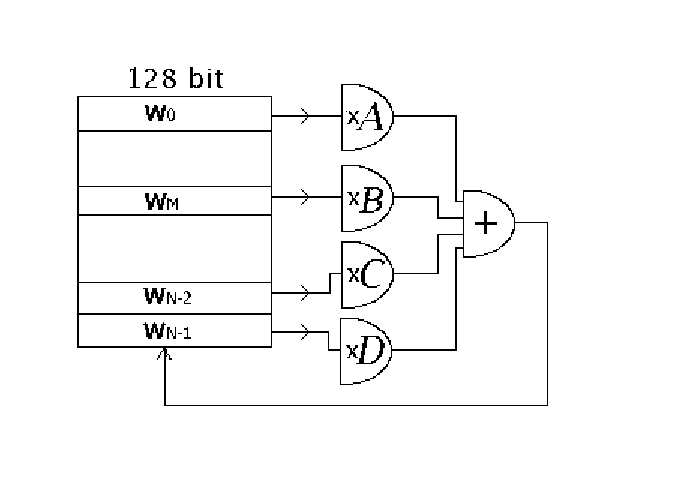
\includegraphics[width=0.7\linewidth]{sfmt-a.eps}
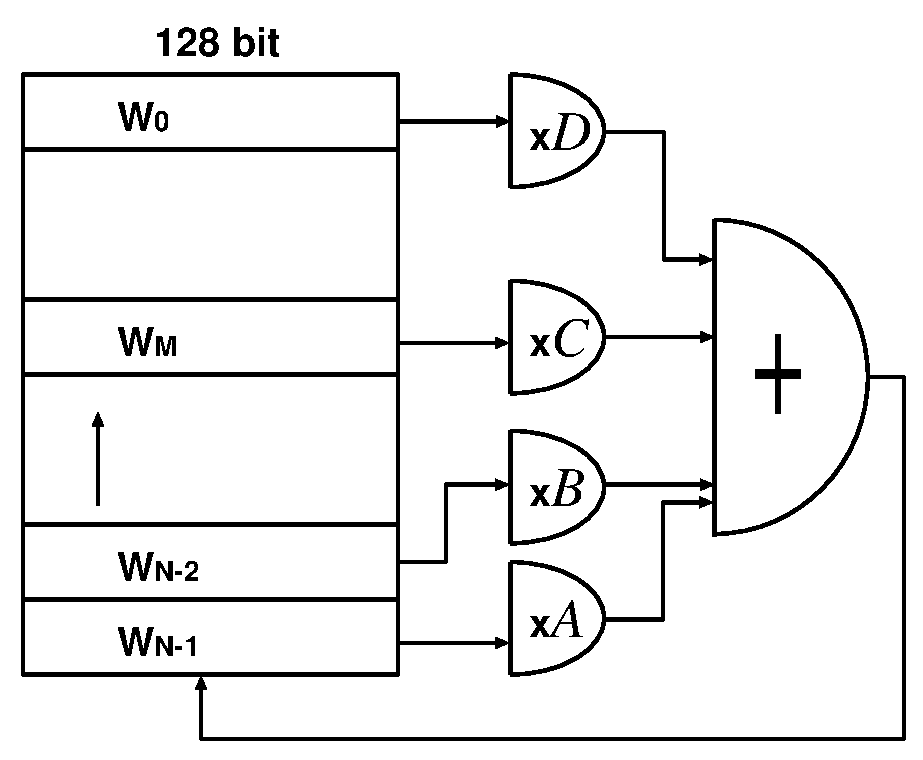
\includegraphics[width=0.7\linewidth]{sfmt-a2.eps}
\\
Figure 6: The transition function of Simple and Fast MT
\end{center}
SFMT is currently implemented for Intel's SSE2 and PowerPC's altivec SIMD
instruction set.

\newpage
Now we provide {\bf fill\_array\_block} interface for the application programs.
INPUT:address of array to fill. This address must be aligned multiple of 16.
INPUT:number of blocks
OUTPUT: the input array is filled by 32-bit pseudo-random numbers.

\newpage
Figure 8 shows an implementation SFMT19937 with period
$2^{19937}-1$.  The function \lshift{128} $n$ is left shift $n$ bit
regarding the word as 128 bit integer, and the function \lshift{32} $n$ is
lesft shift $n$ bit regarding the word as four 32-bit integers
(\rshift{128} and \rshift{32} are shift right).

\begin{center}
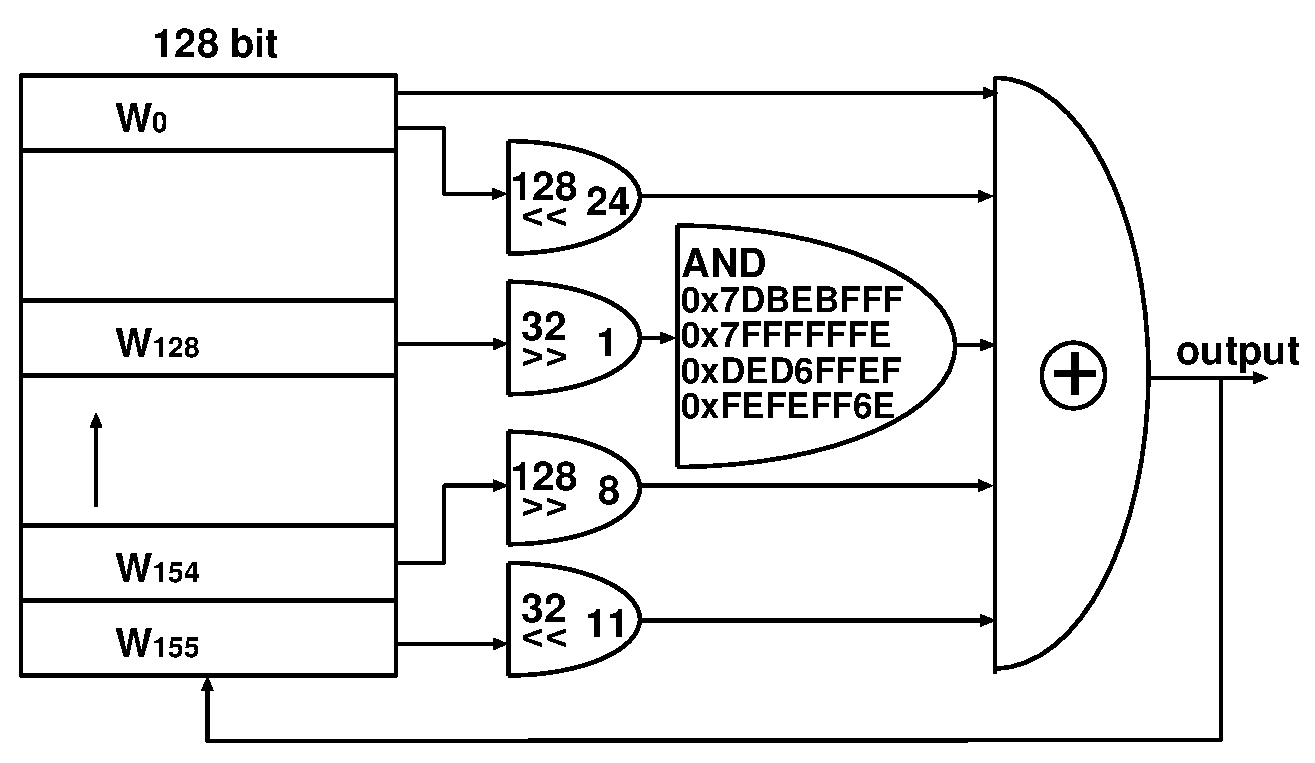
\includegraphics[width=0.7\linewidth]{sfmt-b2.eps}
\\
Figure 8: Detailed description of SFMT19937.
\end{center}


\newpage
\noindent
{\bf 7-2} High dimensional distribution.

{\bf Definition.} 
A periodic sequence with period $P$
$$\bx_0, \bx_1, \ldots, \bx_{P-1}, \bx_P=\bx_0, \ldots$$
of $v$-bit integers is said to be {\em $k$-dimensionally equidistributed}
if any $kv$-bit pattern occurs equally often as a $k$-tuple
$$
(\bx_i, \bx_{i+1}, \ldots, \bx_{i+k-1})
$$
for a period $i=0,\ldots, P-1$. 

(The all-zero pattern occurs once less often.)

\newpage
A periodic sequence of 32-bit integers is said to be
{\em $k$-dimensionally equidistributed with $v$-bit accuracy}
if the most significant $v$ bits of each integer are
$k$-dimensionally equidistributed. 

We denote by $k(v)$ the maximum such $k$. 

\vskip 5mm
We have an upperbound 
$$
k(v) \leq \lfloor \log_2 (P+1) / v \rfloor, 
$$
and define the dimension defect as the summation of the gaps 
$$
\Delta_1 := \sum_{v=1}^{32}(\lfloor \log_2 (P+1) / v \rfloor -k(v)).
$$

\newpage
{\bf 7 Calculate 32-bit $k(v)$ of 128-bit recursion formula PRMG}

\newpage
\noindent
{\bf 7 Comparison of performances}
\\
{\bf 7-1} Compared Generators 
\begin{description}
\item MT19937: Mersenne Twister with period $2^{19937}-1$ ('98).
\end{description}
{\bf 7-1} CPU's
\begin{description}
\item MT19937: Mersenne Twister with period $2^{19937}-1$ ('98).
\end{description}
\newpage

%%%*** change 05/05/10
\newpage
\begin{center}
%\label{table:dist}
\begin{tabular}{|c||c|c|c|c|c|}
\hline
{\Huge Generator}& {\Huge $\Delta_1$} 
  & {\Huge Linux} & {\Huge MacOSX} & {\Huge FreeBSD} & {\Huge Windows} \\ \hline \hline
{\Huge MT19937} & {\Huge 6750}
  & {\Huge 0.92} & {\Huge 1.63} & {\Huge 1.41} & {\Huge 1.42} \\ \hline
{\Huge TT800}  & {\Huge 261} 
  & {\Huge 0.82} & {\Huge 1.51} & {\Huge 1.28} & {\Huge 1.14} \\ \hline
{\Huge XS800} & {\Huge 186}
  & {\Huge 0.79} & {\Huge 1.44} & {\Huge 0.96} & {\Huge 0.89} \\ \hline
{\Huge WELL1024} & {\Huge 0}
  & {\Huge 1.48} & {\Huge 2.23} & {\Huge 1.34} & {\Huge 1.44} \\ \hline
{\Huge WELL44497b} & {\Huge 0}
  & {\Huge 2.13} & {\Huge 3.48} & {\Huge 2.38} & {\Huge 2.52} \\ \hline
{\Huge HT800} & {\Huge 72} 
  & {\Huge 0.95} & {\Huge 1.51} & {\Huge 1.10} & {\Huge 1.02} \\\hline
{\Huge HT1279} & {\Huge 113}
  & {\Huge 0.80} & {\Huge 1.36} & {\Huge 1.06} & {\Huge 0.92} \\ \hline
\end{tabular}
\\
\vskip 5mm
Table 1. Comparison of the dimension defects $\Delta_1$ 
\\
and the time (sec.) to generate $10^8$ prns (gcc -O2). 
\end{center}
%\end{table}

WELL has the optimal equidistribution property, 
but slower than the other generators. 

\newpage
\noindent
{\bf 9 Concluding Remarks}
\begin{itemize}
\item We proposed Hearty Twister. 
\item Faster than Twister GFSR TT800 and WELL.
\item Faster recovery from zero-excess states \\
than TT800 (but inferior to WELL). 
\item Better $k(v)$ than TT800 \\
(but worse than WELL).
\item Better coin-tossing distribution than TT800 \\
(but worse than WELL).
\end{itemize}
We conclude that Hearty Twister is a good compromise
between speed and quality. 

\end{document}




